% If you try this at home, replace the `crinklepaper` with an image of the comet's surface, e.g. from https://arxiv.org/abs/1707.02945
% !TeX program = arara -p generate_examples % | txs:///view-log | txs:///view-pdf "?am).pdf"
\documentclass{standalone}
\usepackage{tikzducks}

\begin{document}

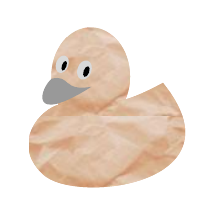
\begin{tikzpicture}[
  path image/.style={
    path picture={
      \foreach \j in {0,...,2}{
        \node at (0,\j) {
          \foreach \i in {1,...,6}{
            \includegraphics[height=2cm]{#1}
          }
        };
      }
    }
  }
]
  \path (0.1,0.1) rectangle (2.1,2.12);
  \begin{pgfinterruptboundingbox}
    \path[path image=crinklepaper] (0.90,1.50) ellipse (0.50 and 0.625);
    \path[path image=crinklepaper] \duckpathbody;
    \fill[gray!80!white] \duckpathbill;
    \fill[white!70!gray, rotate=-20] (0.23,1.7675) ellipse (0.0893 and 0.125) (-0.06,1.74) ellipse (0.0786 and 0.1143);
    \fill[black, rotate=-20] (0.26,1.7575) ellipse (0.0357 and 0.0714) (-0.03,1.73) ellipse (0.0286 and 0.0643);
  \end{pgfinterruptboundingbox}
\end{tikzpicture}

\end{document}